\documentclass[10pt,a4paper,twocolumn]{article}
\usepackage[utf8]{inputenc}
\usepackage[english]{babel}
\usepackage{amsmath}
\usepackage{amsfonts}
\usepackage{amssymb}
\usepackage{graphicx}
\usepackage{geometry}
\usepackage{fancyhdr}
\usepackage{listings}
\usepackage{xcolor}
\usepackage{hyperref}
\usepackage[most]{tcolorbox}
\usepackage{enumitem}
\usepackage{booktabs}
\usepackage{caption}
\usepackage{subcaption}
\usepackage{float}
\usepackage{titlesec}
\usepackage{microtype}
\usepackage{parskip}

% Geometry settings
\geometry{
    a4paper,
    top=2cm,
    bottom=2cm,
    left=1.5cm,
    right=1.5cm,
    headsep=0.5cm,
    footskip=1cm
}

\setlength{\headheight}{15pt}
\pagestyle{fancy}
\fancyhf{}
\rhead{Lab 03 - Synchronization \& Deadlocks}
\lhead{Software Architecture}
\cfoot{\thepage}

\pagenumbering{arabic}

% Code listing settings
\lstset{
    basicstyle=\ttfamily\scriptsize,
    keywordstyle=\color{blue}\bfseries,
    commentstyle=\color{green!60!black}\itshape,
    stringstyle=\color{red},
    showstringspaces=false,
    breaklines=true,
    breakatwhitespace=true,
    frame=leftline,
    framerule=2pt,
    rulecolor=\color{blue!30},
    backgroundcolor=\color{gray!5},
    numbers=left,
    numberstyle=\tiny\color{gray},
    stepnumber=1,
    numbersep=8pt,
    columns=flexible,
    aboveskip=\medskipamount,
    belowskip=\medskipamount,
    xleftmargin=15pt,
    language=Java
}

% Section formatting
\definecolor{darkblue}{RGB}{0,32,96}

\titleformat{\section}
{\color{darkblue}\normalfont\large\bfseries}
{\thesection}{1em}{}

\titleformat{\subsection}
{\color{darkblue}\normalfont\normalsize\bfseries}
{\thesubsection}{1em}{}

\titleformat{\subsubsection}
{\color{darkblue}\normalfont\small\bfseries}
{\thesubsubsection}{1em}{}

% Custom boxes
\newtcolorbox{conceptbox}[1]{
    colback=blue!5!white,
    colframe=blue!75!black,
    colbacktitle=blue!80!black,
    coltitle=white,
    title={\textbf{#1}},
    fonttitle=\bfseries\small,
    boxrule=0.8pt,
    before skip=8pt,
    after skip=8pt,
    left=4pt,
    right=4pt,
    top=6pt,
    bottom=6pt,
    breakable
}

\newtcolorbox{resultbox}[1]{
    colback=green!5!white,
    colframe=green!75!black,
    colbacktitle=green!80!black,
    coltitle=white,
    title={\textbf{#1}},
    fonttitle=\bfseries\small,
    boxrule=0.8pt,
    before skip=8pt,
    after skip=8pt,
    left=4pt,
    right=4pt,
    top=6pt,
    bottom=6pt,
    breakable
}

\newtcolorbox{note}{
    colback=yellow!10!white,
    colframe=orange!75!black,
    colbacktitle=orange!80!black,
    coltitle=white,
    title={\textbf{Important Note}},
    fonttitle=\bfseries\small,
    boxrule=0.8pt,
    before skip=8pt,
    after skip=8pt,
    left=4pt,
    right=4pt,
    top=6pt,
    bottom=6pt,
    breakable
}

\newtcolorbox{warningbox}{
    colback=red!5!white,
    colframe=red!75!black,
    colbacktitle=red!80!black,
    coltitle=white,
    title={\textbf{Deadlock Warning}},
    fonttitle=\bfseries\small,
    boxrule=0.8pt,
    before skip=8pt,
    after skip=8pt,
    left=4pt,
    right=4pt,
    top=6pt,
    bottom=6pt,
    breakable
}

% List formatting
\setlist[itemize]{leftmargin=15pt, itemsep=2pt, parsep=0pt, topsep=5pt}
\setlist[enumerate]{leftmargin=15pt, itemsep=2pt, parsep=0pt, topsep=5pt}

% Caption formatting
\captionsetup{font=small, labelfont=bf, format=hang, indention=0pt, margin=10pt}

% Hyperref setup
\hypersetup{
    colorlinks=true,
    linkcolor=darkblue,
    urlcolor=darkblue,
    citecolor=darkblue,
    pdfborder={0 0 0}
}

% Title page
\title{\vspace{-1cm}
    \begin{center}
        
\includegraphics[width=0.25\textwidth]{media/university_logo.png}
    \end{center}
    \vspace{1.5cm}
    \textbf{\Large Software Architecture Laboratory}\\
    \vspace{1cm}
    \textbf{\huge Laboratory No. 3}\\
    \textbf{\huge Synchronization \& Deadlocks}\\
    \vspace{1.5cm}
    \large Immortals Simulation with Java 21
}

\author{
    \vspace{2cm}
    \textbf{Students:}\\[0.05cm]
    Andersson David S\'{a}nchez M\'{e}ndez\\[0.3cm]
    Cristian Santiago Pedraza Rodr\'{i}guez\\[0.3cm]
    Elizabeth Correa Su\'{a}rez\\[0.3cm]
    Juan Sebastian Ortega Mu\~{n}oz\\[1.5cm]
    \textbf{Instructor:} Professor Javier Ivan Toquica Barrera\\[0.5cm]
    \textbf{Course:} Software Architecture (ARSW)\\[0.3cm]
    \textbf{Institution:} Escuela Colombiana de Ingenier\'{i}a Julio Garavito\\[2cm]
}

\date{February 13, 2026}

\begin{document}

\onecolumn
\maketitle
\thispagestyle{empty}
\newpage

\tableofcontents
\newpage

\twocolumn

% ============================================
\section{Objective}
% ============================================

This laboratory focuses on practicing minimal synchronization, avoiding deadlocks, and implementing cooperative suspension in an ``immortals''-type thread system using Java 21. The simulation involves multiple concurrent threads representing immortal warriors that fight each other, requiring proper coordination to ensure correct behavior and data consistency.

The specific goals include:

\begin{itemize}
    \item \textbf{Producer/Consumer}: Implement efficient CPU usage with \texttt{wait()}/\texttt{notify()} instead of busy-wait.
    \item \textbf{Distributed Search}: Implement early termination and atomic counters without race conditions.
    \item \textbf{Deadlock Prevention}: Identify and fix deadlocks using total order or \texttt{tryLock(timeout)}.
    \item \textbf{Pause/Resume Control}: Implement stable pause mechanism with synchronization barriers.
    \item \textbf{Thread-safe Collections}: Handle concurrent modifications without blocking the simulation.
    \item \textbf{Orderly Shutdown}: Implement graceful termination of all threads.
\end{itemize}

% ============================================
\section{Problem Description}
% ============================================

The immortals simulator presents several concurrency challenges across three main parts:

\begin{warningbox}
\begin{enumerate}
    \item \textbf{Part I - Busy-Wait}: High CPU consumption in producer/consumer due to spin-wait pattern.
    \item \textbf{Part II - Race Conditions}: Distributed search with shared counter may have race conditions.
    \item \textbf{Part III - Deadlocks}: Multiple immortals acquiring nested locks may cause circular wait.
\end{enumerate}
\end{warningbox}

\subsection{Application Architecture}

The application follows a layered architecture:

\begin{table}[H]
    \centering
    \small
    \begin{tabular}{|l|l|}
        \hline
        \textbf{Package} & \textbf{Responsibility} \\
        \hline
        \texttt{app} & Bootstrap (Main) \\
        \hline
        \texttt{highlandersim} & Swing UI \\
        \hline
        \texttt{immortals} & Domain model \\
        \hline
        \texttt{concurrency} & PauseController \\
        \hline
        \texttt{demos} & Theoretical demos \\
        \hline
        \texttt{core} & Bank transfers \\
        \hline
    \end{tabular}
    \caption{Application package structure}
    \label{tab:packages}
\end{table}

% ============================================
\section{Theoretical Framework}
% ============================================

\subsection{Busy-Wait vs Wait/Notify}

\textbf{Busy-wait} (spin-wait) is a pattern where a thread continuously checks a condition in a tight loop:

\begin{lstlisting}[caption={Busy-Wait Pattern (Inefficient)}]
while (true) {
    if (queue.size() < capacity) {
        queue.add(item);
        return;
    }
    Thread.onSpinWait(); // CPU spinning!
}
\end{lstlisting}

The \texttt{wait()}/\texttt{notify()} pattern releases CPU when waiting:

\begin{lstlisting}[caption={Wait/Notify Pattern (Efficient)}]
synchronized (this) {
    while (queue.size() == capacity) {
        this.wait(); // Release CPU
    }
    queue.add(item);
    this.notifyAll();
}
\end{lstlisting}

\begin{conceptbox}{Wait/Notify Semantics}
\begin{itemize}
    \item \texttt{wait()}: Releases lock, enters WAITING state
    \item \texttt{notify()}: Wakes one waiting thread
    \item \texttt{notifyAll()}: Wakes all waiting threads
    \item Use \texttt{while} loop for spurious wakeups
\end{itemize}
\end{conceptbox}

\subsection{Deadlock Conditions}

A \textbf{deadlock} occurs when four conditions hold simultaneously:

\begin{enumerate}
    \item \textbf{Mutual Exclusion}: Resources cannot be shared.
    \item \textbf{Hold and Wait}: Thread holds one resource while waiting for another.
    \item \textbf{No Preemption}: Resources cannot be forcibly taken.
    \item \textbf{Circular Wait}: Threads form a circular chain of waiting.
\end{enumerate}

\subsection{Deadlock Prevention Strategies}

\textbf{Strategy 1: Total Order}

\begin{lstlisting}[caption={Total Order Lock Acquisition}]
Immortal first = name.compareTo(
    other.name) < 0 ? this : other;
Immortal second = name.compareTo(
    other.name) < 0 ? other : this;
synchronized (first) {
  synchronized (second) {
    // Critical section
  }
}
\end{lstlisting}

\textbf{Strategy 2: TryLock with Timeout}

\begin{lstlisting}[caption={TryLock with Backoff}]
if (this.lock.tryLock(10, MILLISECONDS)) {
  try {
    if (other.lock.tryLock(10, MILLISECONDS)) {
      try {
        // Critical section
      } finally {
        other.lock.unlock();
      }
    }
  } finally {
    this.lock.unlock();
  }
}
// Exponential backoff on failure
\end{lstlisting}

% ============================================
\section{Part I: Producer/Consumer}
% ============================================

\subsection{Problem: High CPU Consumption}

The \texttt{BusySpinQueue} class implements a busy-wait pattern that causes excessive CPU usage:

\begin{lstlisting}[caption={BusySpinQueue - High CPU}]
// take method - CPU spinning
while (true) {
    T v = q.pollFirst();
    if (v != null) return v;
    Thread.onSpinWait(); // Keeps CPU busy
}
\end{lstlisting}

\subsection{Evidence of High CPU Usage}

\begin{figure}[H]
    \centering
    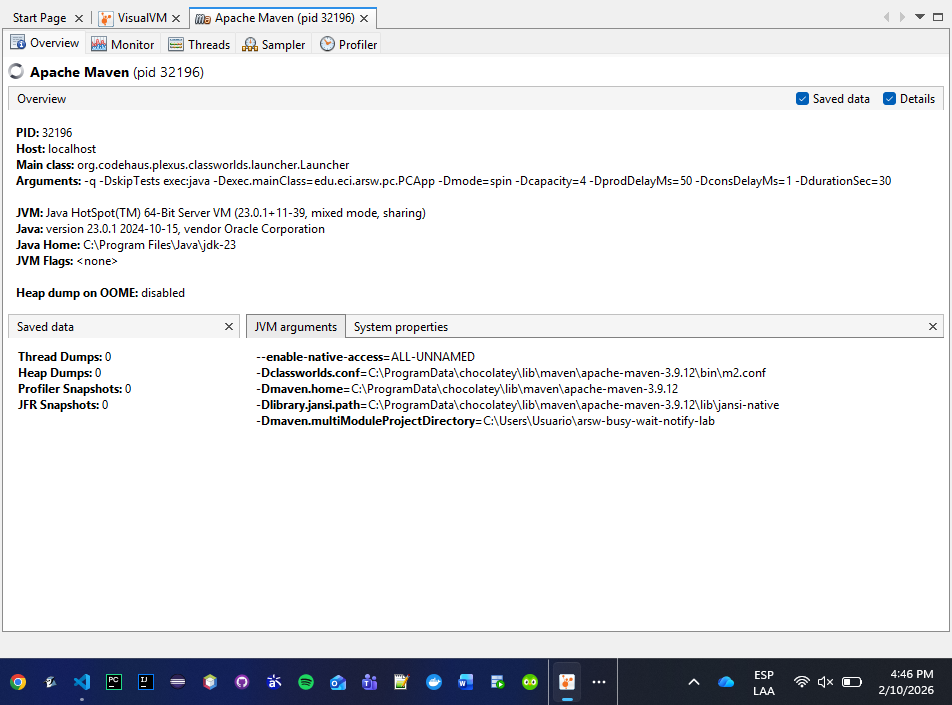
\includegraphics[width=0.45\textwidth]{../images/first_screenshot.png}
    \caption{jVisualVM Monitor: High CPU usage with busy-wait (spin mode).}
\end{figure}

\begin{figure}[H]
    \centering
    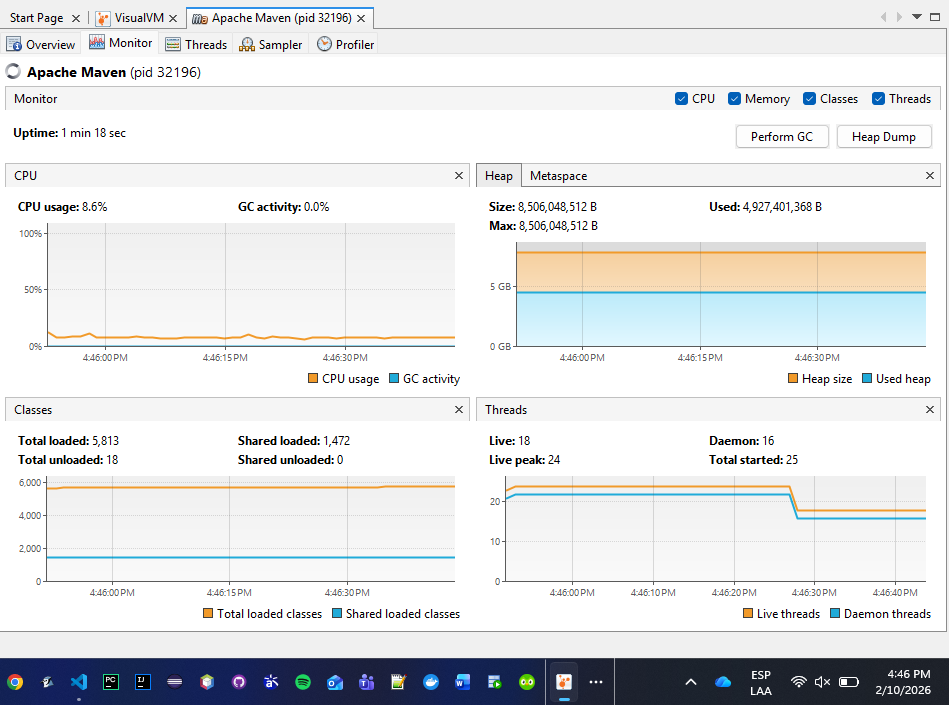
\includegraphics[width=0.45\textwidth]{../images/second_screenshot.png}
    \caption{jVisualVM Threads: Threads constantly in RUNNABLE state.}
\end{figure}

\subsection{Solution: BoundedBuffer with Monitors}

\begin{lstlisting}[caption={BoundedBuffer - Efficient CPU}]
public T take() throws InterruptedException {
    synchronized (this) {
        while (q.isEmpty()) {
            this.wait(); // Release CPU
        }
        T v = q.removeFirst();
        this.notifyAll();
        return v;
    }
}
\end{lstlisting}

\begin{lstlisting}[caption={BoundedBuffer - Put Method}]
public void put(T item) 
    throws InterruptedException {
    synchronized (this) {
        while (q.size() == capacity) {
            this.wait(); // Wait when full
        }
        q.addLast(item);
        this.notifyAll();
    }
}
\end{lstlisting}

\subsection{Evidence of Efficient CPU Usage}

\begin{figure}[H]
    \centering
    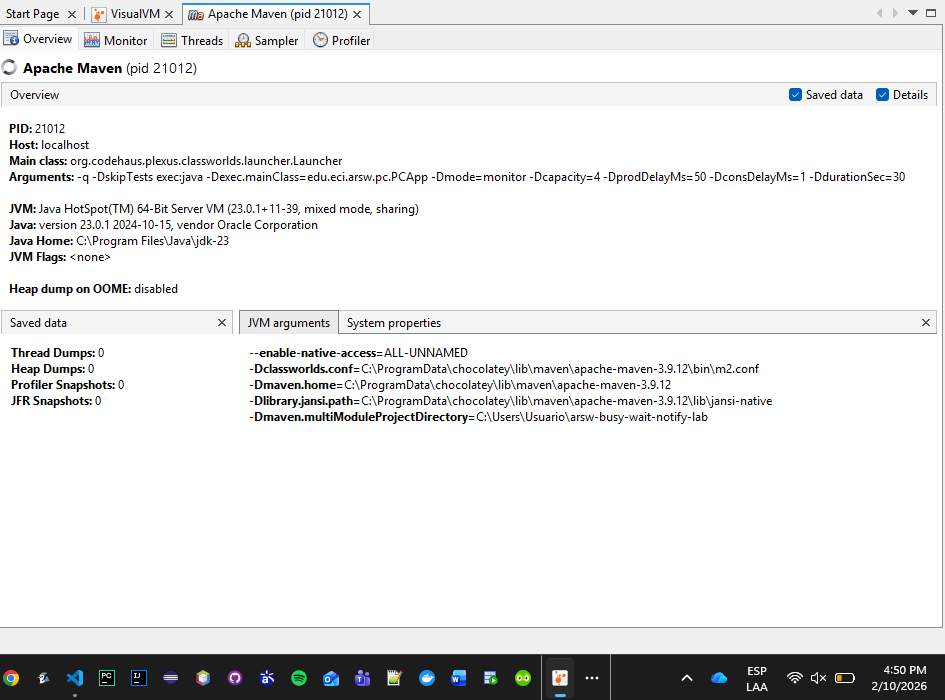
\includegraphics[width=0.45\textwidth]{../images/third_screenshot.png}
    \caption{jVisualVM Monitor: Low CPU usage with monitors.}
\end{figure}

\begin{figure}[H]
    \centering
    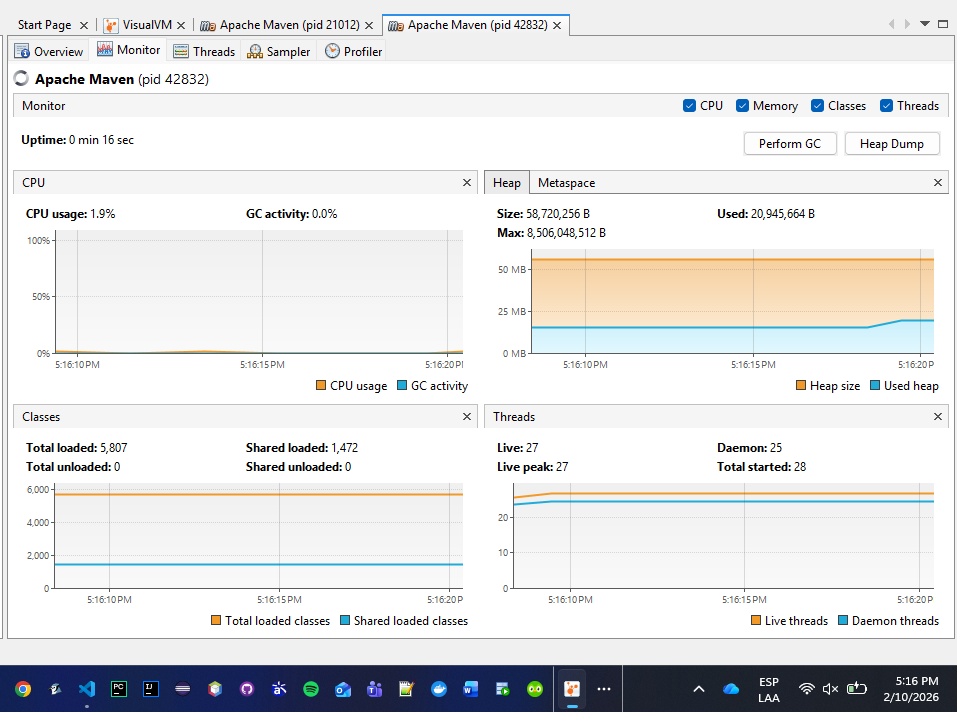
\includegraphics[width=0.45\textwidth]{../images/fourth-screenshot.png}
    \caption{jVisualVM Threads: Threads in WAITING state when idle.}
\end{figure}

\subsection{Fast Producer / Slow Consumer}

When the producer is faster than the consumer with a bounded queue:

\begin{figure}[H]
    \centering
    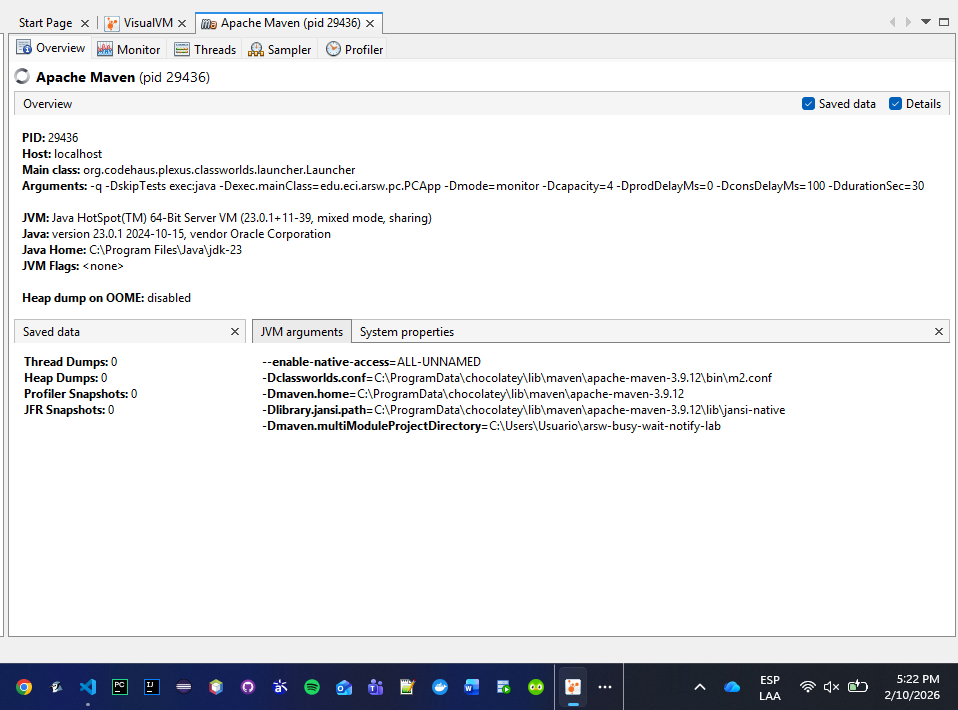
\includegraphics[width=0.45\textwidth]{../images/fifth_screenshot.png}
    \caption{Producer waits efficiently when queue is full.}
\end{figure}

\begin{figure}[H]
    \centering
    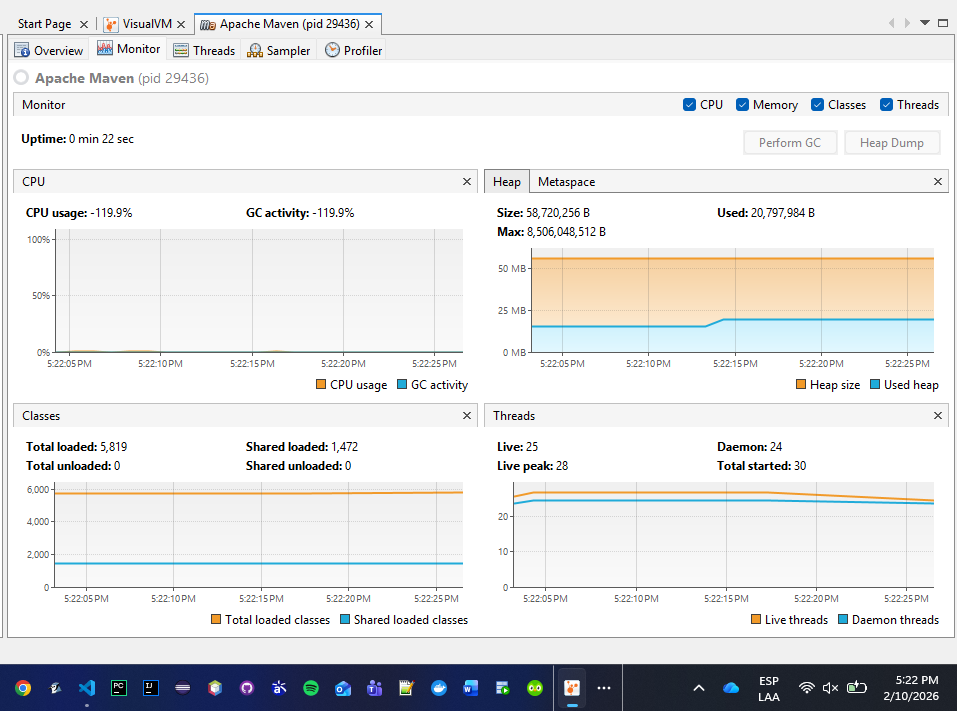
\includegraphics[width=0.45\textwidth]{../images/sixth_screenshot.png}
    \caption{Producer in WAITING state when queue reaches capacity.}
\end{figure}

% ============================================
\section{Part II: Distributed Search}
% ============================================

\subsection{Early Stop Implementation}

The distributed search pattern was adapted to the greyhound race domain:

\begin{table}[H]
    \centering
    \small
    \begin{tabular}{|l|l|}
        \hline
        \textbf{Concept} & \textbf{Dogs Race} \\
        \hline
        Search threads & Galgo threads \\
        \hline
        Occurrence counter & AtomicInteger \\
        \hline
        ALARM\_COUNT & arrivalAlarmCount \\
        \hline
    \end{tabular}
    \caption{Mapping to distributed search pattern}
    \label{tab:mapping}
\end{table}

\subsection{AtomicInteger for Race-Free Counting}

\begin{lstlisting}[caption={Atomic Counter - No Race Condition}]
// BEFORE: Race condition possible
final int position = nextPosition++;

// AFTER: Atomic CAS operation
final int position = 
    nextPosition.getAndIncrement();
\end{lstlisting}

\subsection{Early Stop Check}

\begin{lstlisting}[caption={Early Stop in Thread Loop}]
while (paso < carril.size()) {
    control.awaitIfPaused();
    
    // Early-stop check
    if (registry.hasReachedThreshold()) {
        stoppedEarly = true;
        break; // Don't traverse remaining
    }
    // ... continue stepping
}
\end{lstlisting}

\subsection{Evidence of Early Stop}

\begin{figure}[H]
    \centering
    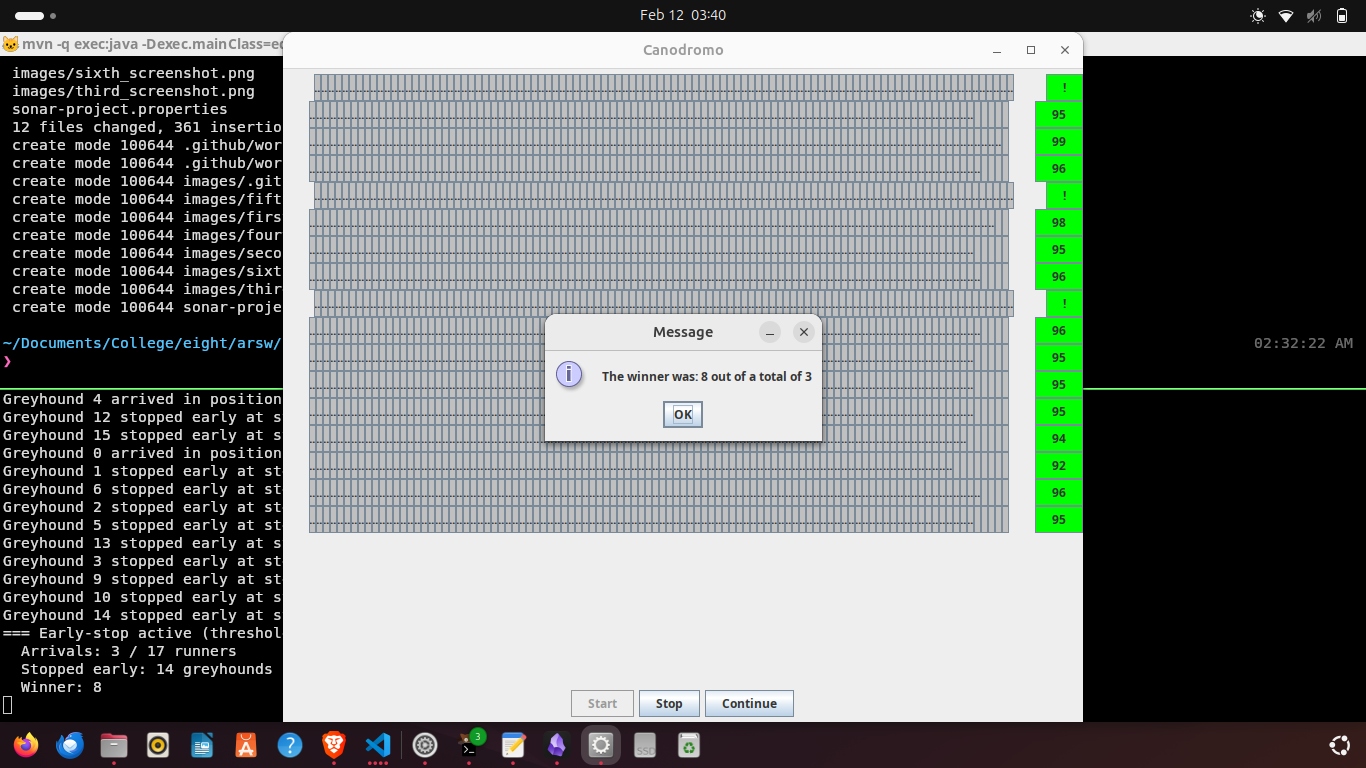
\includegraphics[width=0.45\textwidth]{../images/part2-first-execution.png}
    \caption{With threshold=3: Race stops after 3 arrivals.}
\end{figure}

\begin{figure}[H]
    \centering
    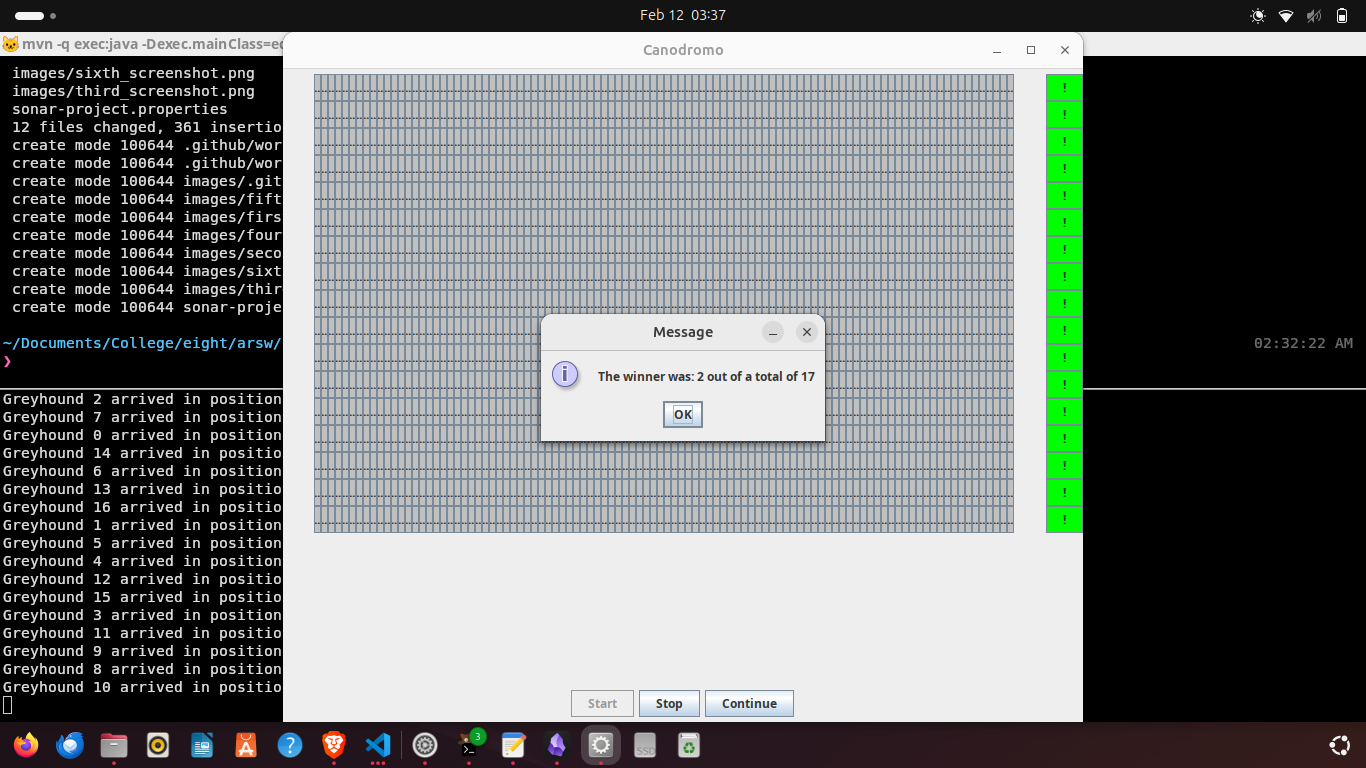
\includegraphics[width=0.45\textwidth]{../images/part2-second-execution.png}
    \caption{Without threshold: All 17 greyhounds finish.}
\end{figure}

% ============================================
\section{Part III: Immortals Simulation}
% ============================================

\subsection{Simulation Overview}

The simulation models $N$ immortals running concurrently. Each immortal is represented by one thread and repeatedly attacks another immortal:

\begin{itemize}
    \item $N$: number of immortals (\texttt{-Dcount})
    \item $H$: initial health (\texttt{-Dhealth})
    \item $M$: damage per hit (\texttt{-Ddamage})
\end{itemize}

\textbf{Fight rule:}
\begin{itemize}
    \item Attacker decreases opponent health by $M$
    \item Attacker increases own health by $M/2$
\end{itemize}

\subsection{Invariant Calculation}

Initial total health:
$$S_0 = N \cdot H = 8 \cdot 100 = 800$$

Change per fight:
$$\Delta = -M + \frac{M}{2} = -10 + 5 = -5$$

After $k$ fights:
$$S(k) = S_0 + k\Delta = 800 - 5k$$

\begin{note}
The constant invariant ($N \times H$) is \textbf{not} maintained because each fight reduces the global total by $M/2$. However, the implementation-based invariant $S(k) = S_0 - 5k$ is maintained.
\end{note}

\subsection{Pause \& Check Validation}

\begin{figure}[H]
    \centering
    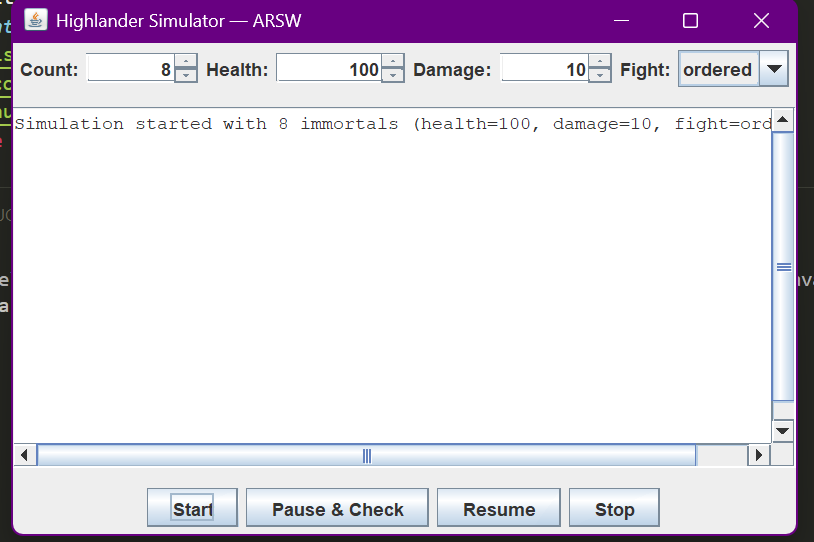
\includegraphics[width=0.45\textwidth]{../images/imagen2.png}
    \caption{Pause \& Check showing Score=146, Total Health=70.}
\end{figure}

Using the formula: $S(146) = 800 - 5(146) = 70$ --- matches observed value!

\begin{figure}[H]
    \centering
    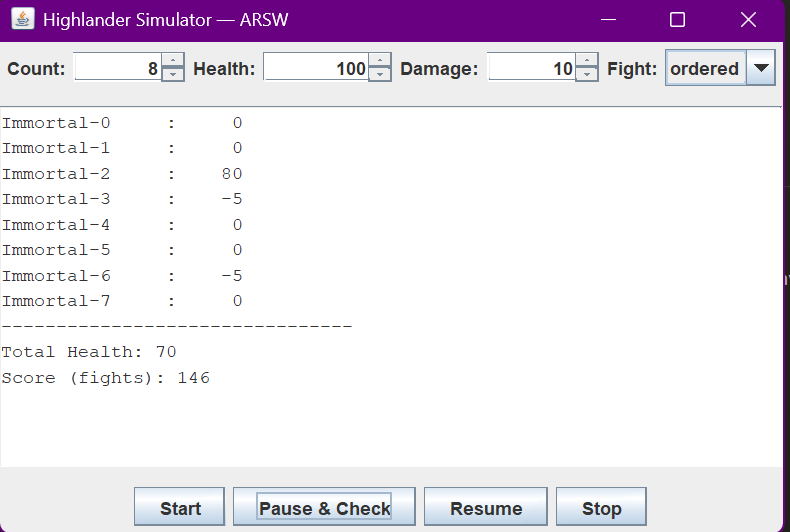
\includegraphics[width=0.45\textwidth]{../images/imagen1.png}
    \caption{Detailed health breakdown per immortal.}
\end{figure}

\subsection{Multiple Pause Validation}

\begin{table}[H]
    \centering
    \small
    \begin{tabular}{|c|c|c|c|}
        \hline
        \textbf{Pause} & \textbf{Score} & \textbf{Observed} & \textbf{Expected} \\
        \hline
        1 & 1712 & 2864 & $8000-3(1712)$ \\
        \hline
        2 & 2575 & 275 & $8000-3(2575)$ \\
        \hline
        3 & 2648 & 56 & $8000-3(2648)$ \\
        \hline
    \end{tabular}
    \caption{Multiple pause validation (all match)}
    \label{tab:pause}
\end{table}

\begin{figure}[H]
    \centering
    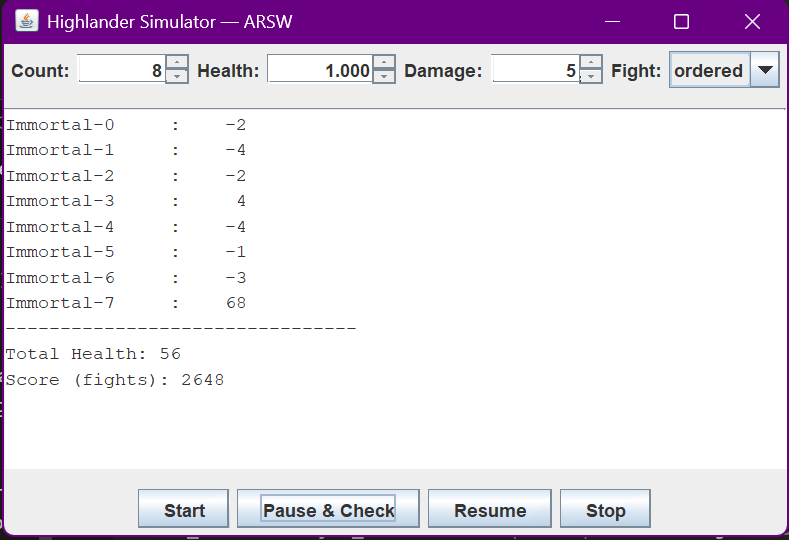
\includegraphics[width=0.45\textwidth]{../images/test1.png}
    \caption{Pause test with k=2648, observed total=56.}
\end{figure}

% ============================================
\section{Deadlock Analysis}
% ============================================

\subsection{Critical Sections Identified}

The main critical section is the fight operation:

\begin{lstlisting}[caption={Critical Section - Fight Operation}]
other.health -= this.damage;    // Write
this.health += this.damage / 2; // Write
scoreBoard.recordFight();       // Update
\end{lstlisting}

\subsection{Naive Strategy (Causes Deadlock)}

\begin{lstlisting}[caption={Naive Lock Acquisition}]
synchronized (this) {           
  synchronized (other) {        
    // Fight logic
  }
}
\end{lstlisting}

\textbf{The deadlock scenario:}
\begin{verbatim}
Thread A (5 vs 3):   Thread B (3 vs 5):
  Lock(5) OK           Lock(3) OK
  wants(3) BLOCKED     wants(5) BLOCKED
  --> DEADLOCK <--
\end{verbatim}

\begin{figure}[H]
    \centering
    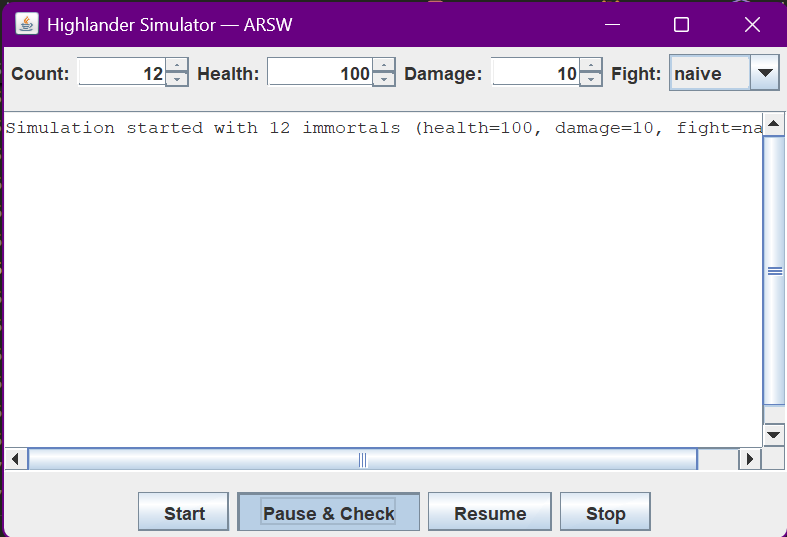
\includegraphics[width=0.45\textwidth]{../images/UInaive.png}
    \caption{UI frozen with naive mode after a few seconds.}
\end{figure}

\begin{figure}[H]
    \centering
    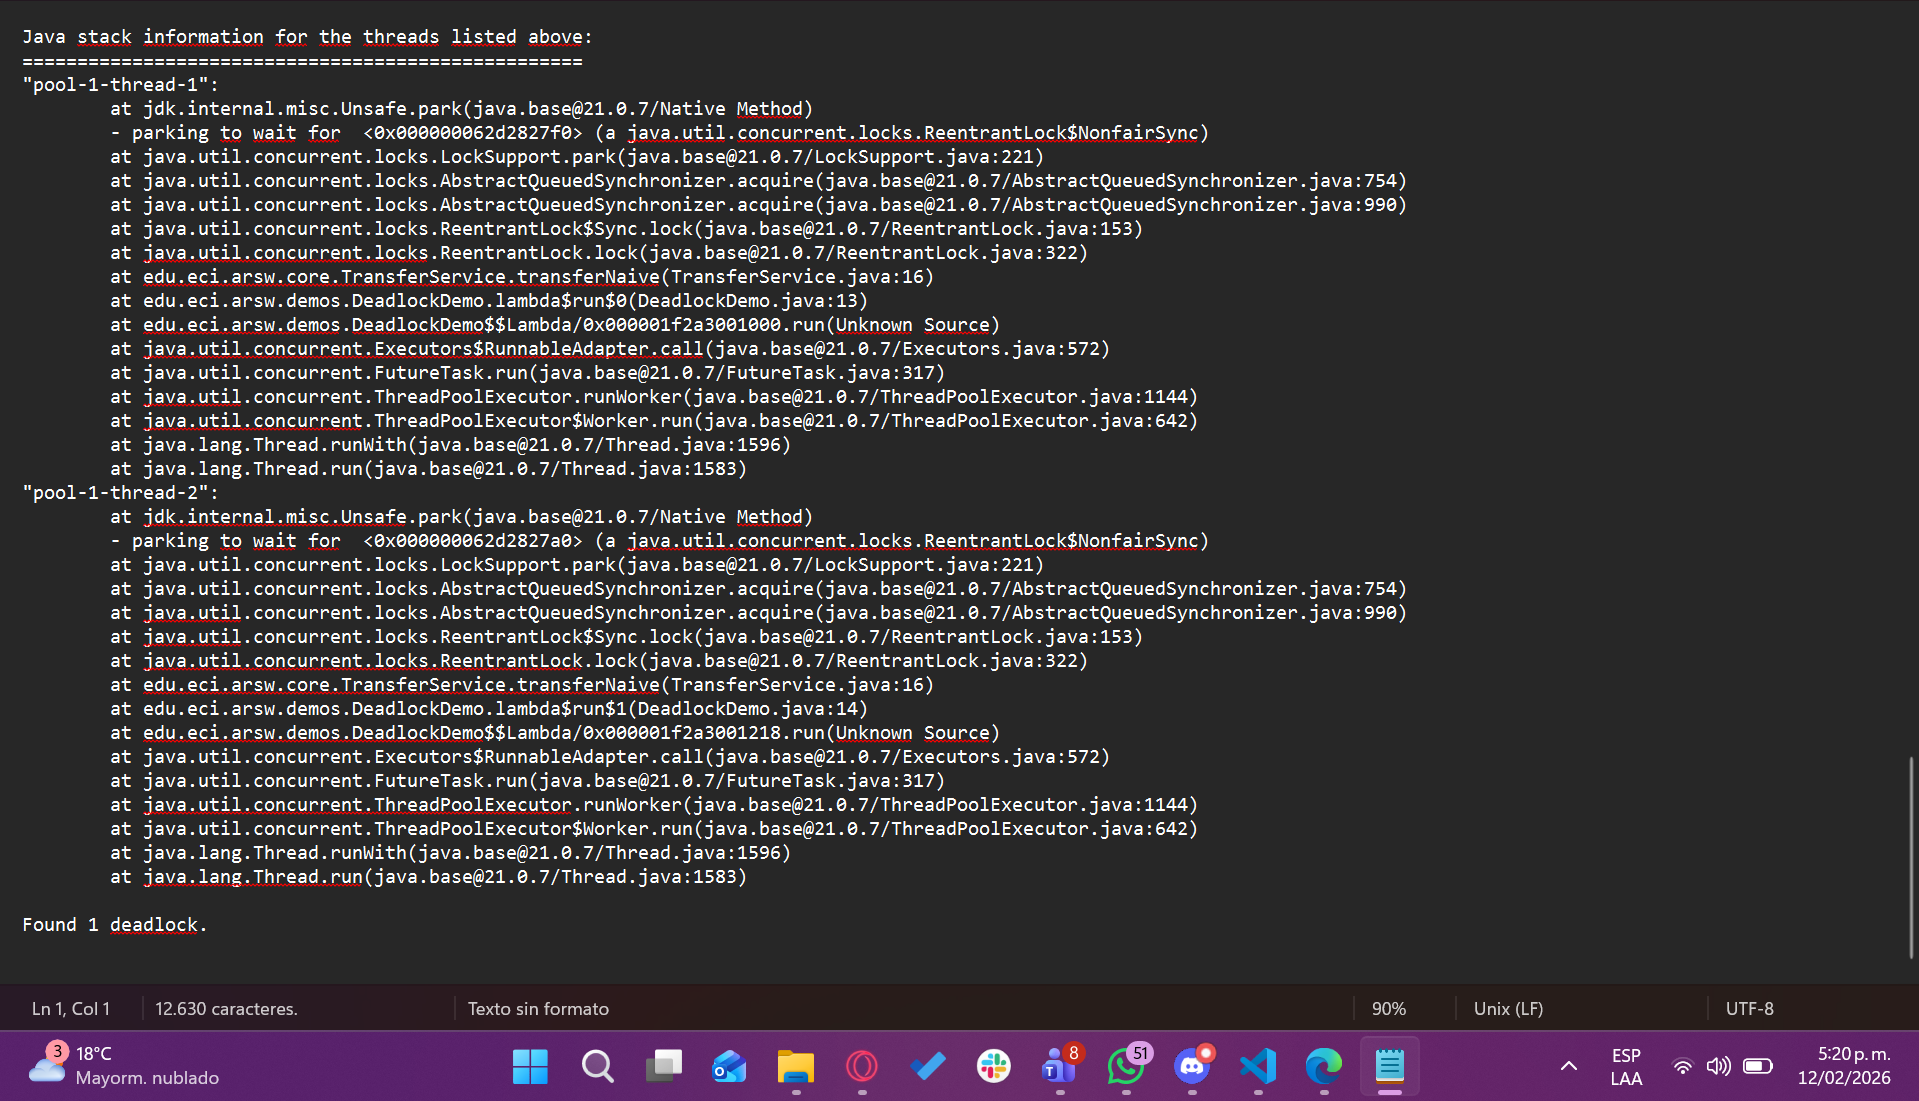
\includegraphics[width=0.45\textwidth]{../images/naive.png}
    \caption{jstack output confirms deadlock.}
\end{figure}

\subsection{Ordered Strategy (No Deadlock)}

\begin{lstlisting}[caption={Ordered Lock Acquisition}]
Immortal first = this.name.compareTo(
    other.name) < 0 ? this : other;
Immortal second = this.name.compareTo(
    other.name) < 0 ? other : this;
synchronized (first) {
  synchronized (second) {
    // Fight logic
  }
}
\end{lstlisting}

\begin{figure}[H]
    \centering
    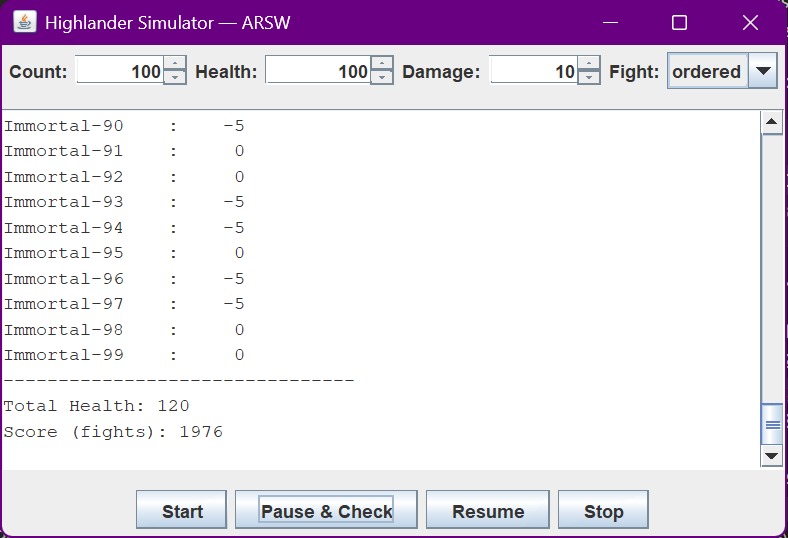
\includegraphics[width=0.45\textwidth]{../images/UIordered.png}
    \caption{UI remains responsive with ordered mode.}
\end{figure}

\begin{figure}[H]
    \centering
    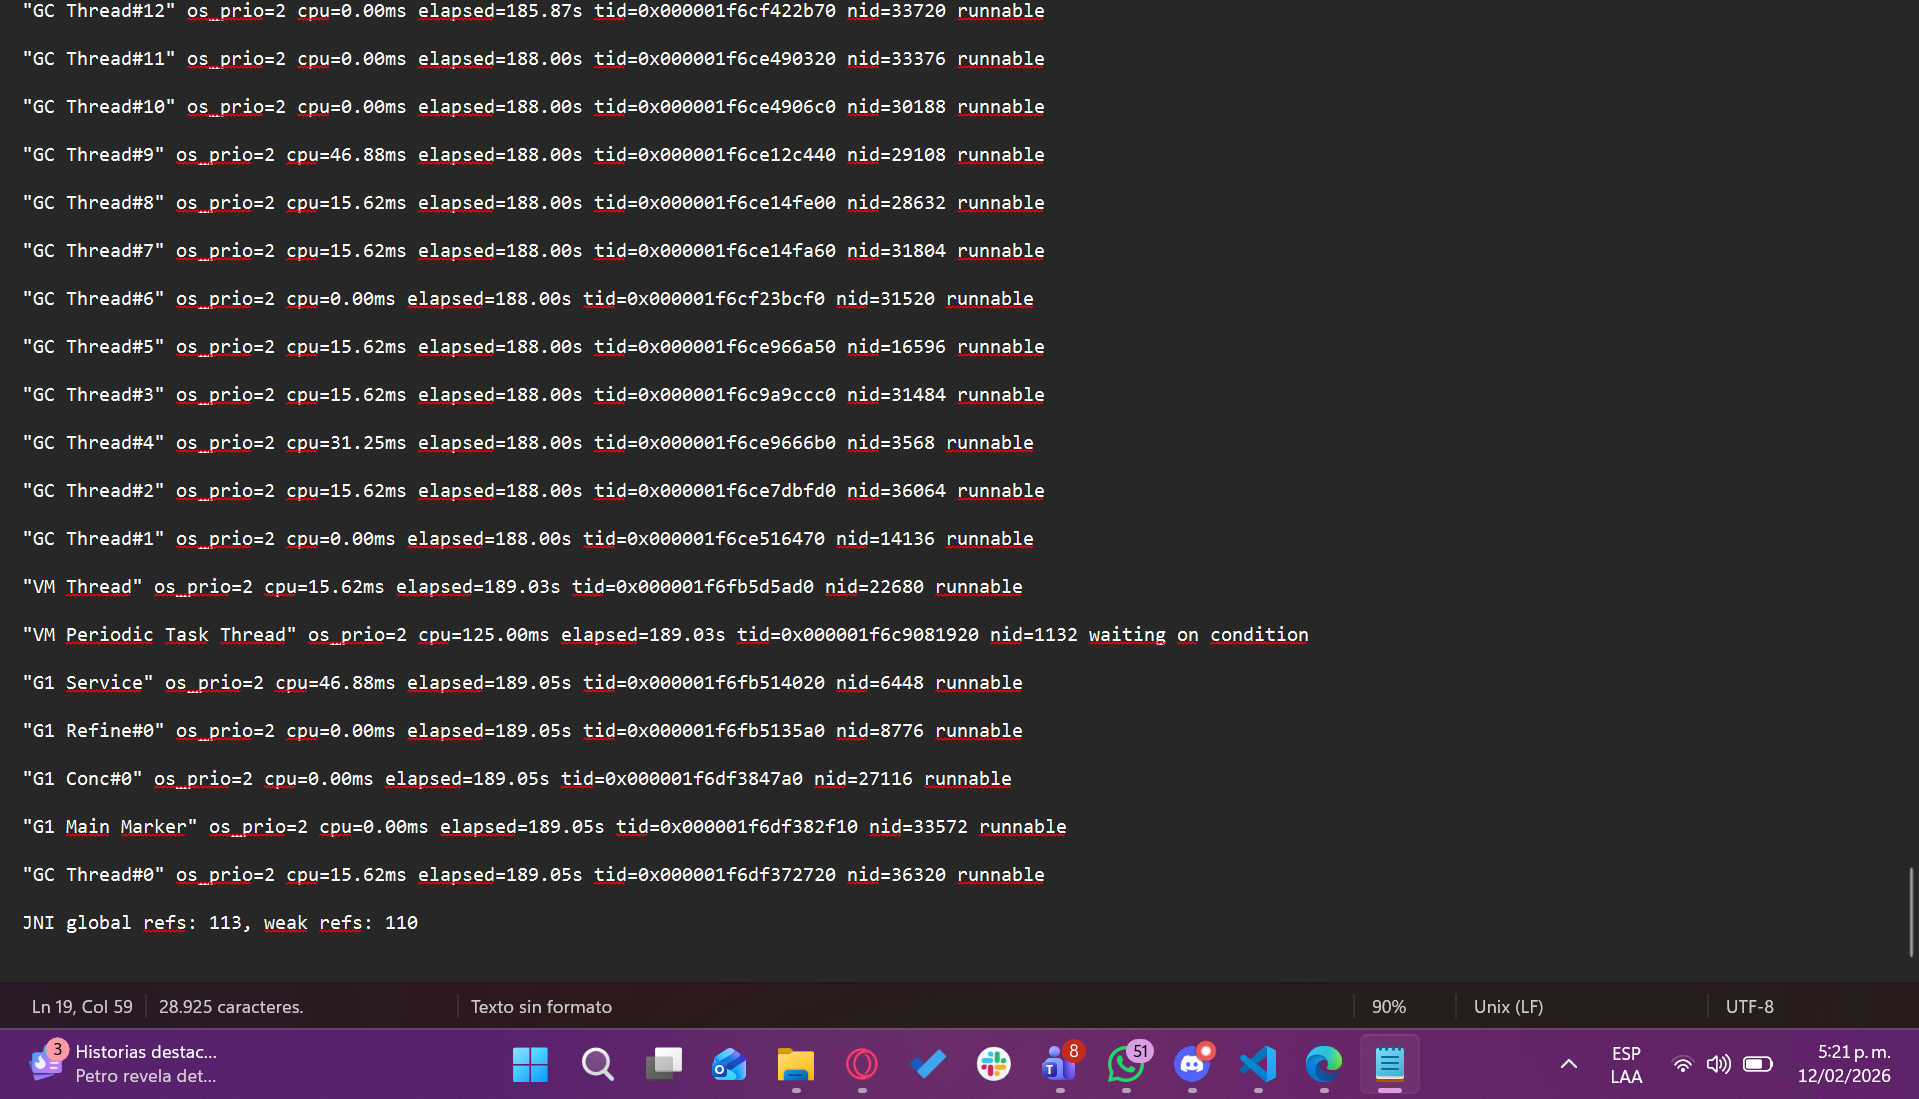
\includegraphics[width=0.45\textwidth]{../images/ordered.png}
    \caption{jstack shows no deadlock with ordered mode.}
\end{figure}

\subsection{TryLock with Exponential Backoff}

\begin{lstlisting}[caption={TryLock Strategy}]
for (int attempt = 0; 
     attempt < MAX_RETRIES; attempt++) {
  if (this.lock.tryLock(10, MILLISECONDS)) {
    try {
      if (other.lock.tryLock(10, MILLISECONDS)) {
        try {
          // Fight logic
          return; // Success
        } finally { other.lock.unlock(); }
      }
    } finally { this.lock.unlock(); }
  }
  // Exponential backoff with jitter
  Thread.sleep(backoff + jitter);
  backoff = Math.min(backoff * 2, MAX_BACKOFF);
}
\end{lstlisting}

\subsection{Strategy Comparison}

\begin{table}[H]
    \centering
    \scriptsize
    \begin{tabular}{|l|c|c|c|}
        \hline
        \textbf{Aspect} & \textbf{Naive} & \textbf{Ordered} & \textbf{TryLock} \\
        \hline
        Lock mechanism & synch & synch & ReentrantLock \\
        \hline
        Lock order & this$\to$other & alphabetical & any \\
        \hline
        Deadlock? & YES & NO & NO \\
        \hline
        Livelock? & NO & NO & NO \\
        \hline
        Blocking & infinite & infinite & timeout \\
        \hline
    \end{tabular}
    \caption{Fight strategy comparison}
    \label{tab:strategies}
\end{table}

% ============================================
\section{High N Validation}
% ============================================

\subsection{N=100 Results}

\begin{figure}[H]
    \centering
    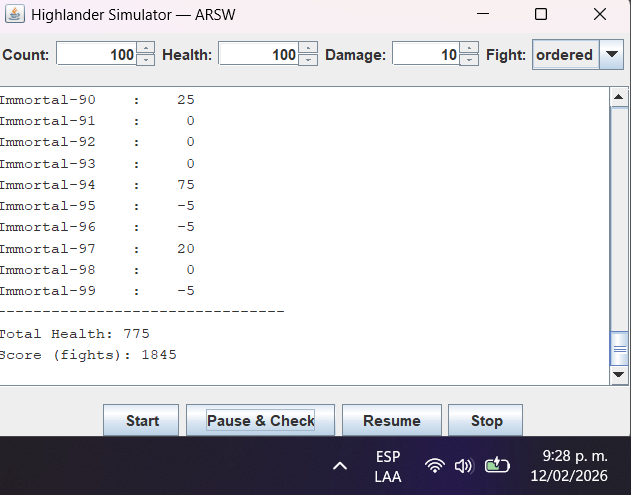
\includegraphics[width=0.45\textwidth]{../images/validation_n100_ordered.png}
    \caption{Validation N=100 with ordered strategy.}
\end{figure}

\begin{figure}[H]
    \centering
    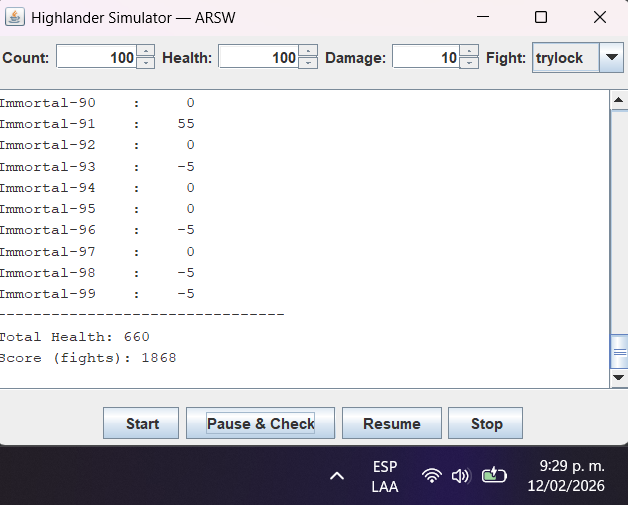
\includegraphics[width=0.45\textwidth]{../images/validation_n100_trylock.png}
    \caption{Validation N=100 with trylock strategy.}
\end{figure}

\subsection{N=1000 Results}

\begin{figure}[H]
    \centering
    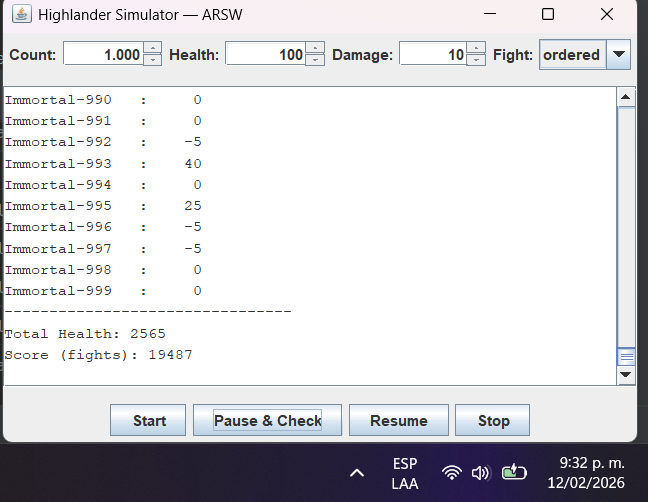
\includegraphics[width=0.45\textwidth]{../images/validation_n1000_ordered.png}
    \caption{Validation N=1000 with ordered strategy.}
\end{figure}

\begin{figure}[H]
    \centering
    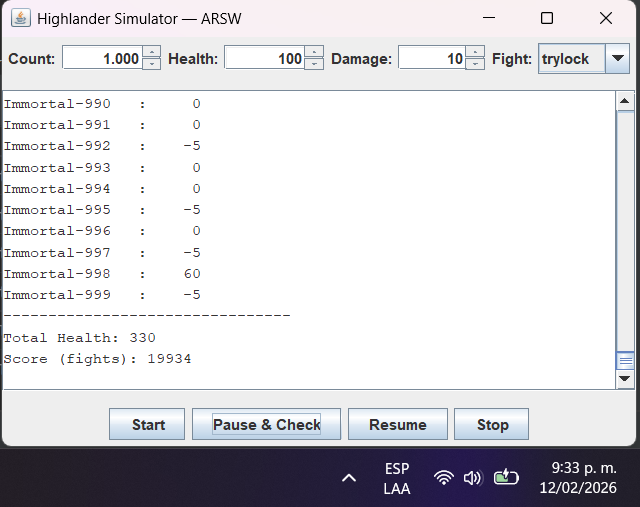
\includegraphics[width=0.45\textwidth]{../images/validation_n1000_trylock.png}
    \caption{Validation N=1000 with trylock strategy.}
\end{figure}

\subsection{N=10000 Results}

\begin{figure}[H]
    \centering
    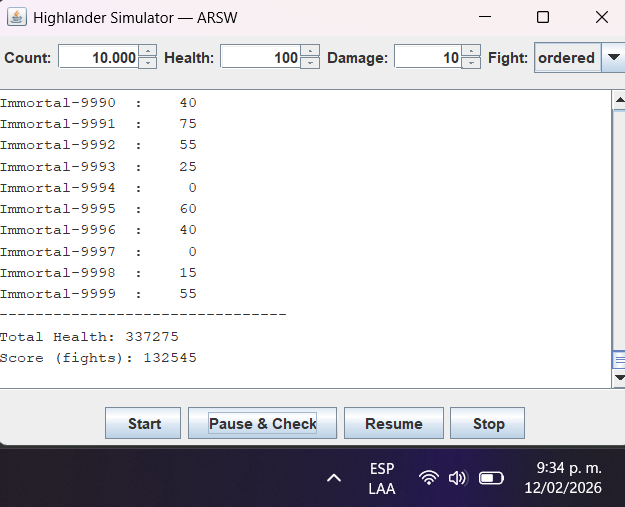
\includegraphics[width=0.45\textwidth]{../images/validation_n10000_ordered.png}
    \caption{Validation N=10000 with ordered strategy.}
\end{figure}

\begin{figure}[H]
    \centering
    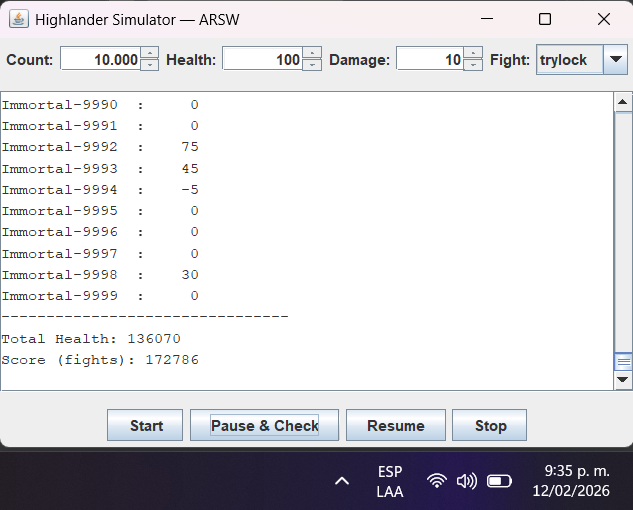
\includegraphics[width=0.45\textwidth]{../images/validation_n10000_trylock.png}
    \caption{Validation N=10000 with trylock strategy.}
\end{figure}

\subsection{Validation Summary}

\begin{table}[H]
    \centering
    \scriptsize
    \begin{tabular}{|c|c|c|c|c|}
        \hline
        \textbf{N} & \textbf{Strategy} & \textbf{Score} & \textbf{Total} & \textbf{Match?} \\
        \hline
        100 & ordered & 1845 & 775 & $\checkmark$ \\
        \hline
        100 & trylock & 1868 & 660 & $\checkmark$ \\
        \hline
        1000 & ordered & 19487 & 2565 & $\checkmark$ \\
        \hline
        1000 & trylock & 19934 & 330 & $\checkmark$ \\
        \hline
        10000 & ordered & 132545 & 337275 & $\checkmark$ \\
        \hline
        10000 & trylock & 172786 & 136070 & $\checkmark$ \\
        \hline
    \end{tabular}
    \caption{High N validation results}
    \label{tab:highN}
\end{table}

% ============================================
\section{Removing Dead Immortals}
% ============================================

\subsection{Problem: Race Conditions with ArrayList}

The original implementation used \texttt{ArrayList<Immortal>} which causes:

\begin{itemize}
    \item \texttt{ConcurrentModificationException} during iteration
    \item \texttt{IndexOutOfBoundsException} on concurrent access
    \item Stale size values
\end{itemize}

\subsection{Solution: CopyOnWriteArrayList}

\texttt{CopyOnWriteArrayList} provides thread-safe operations:

\begin{lstlisting}[caption={Lock-Free Collection}]
private final List<Immortal> population = 
    new CopyOnWriteArrayList<>();
\end{lstlisting}

\textbf{Key properties:}
\begin{itemize}
    \item Thread-safe without explicit synchronization
    \item Snapshot iteration (no CME)
    \item Lock-free reads
    \item Copy-on-write semantics
\end{itemize}

\begin{table}[H]
    \centering
    \scriptsize
    \begin{tabular}{|l|c|c|}
        \hline
        \textbf{Aspect} & \textbf{ArrayList+sync} & \textbf{COWAL} \\
        \hline
        Reads & Blocked & Lock-free \\
        \hline
        Writes & Fast+lock & Slower (copy) \\
        \hline
        Iteration & Requires sync & Safe \\
        \hline
        Best for & Frequent writes & Frequent reads \\
        \hline
    \end{tabular}
    \caption{Collection comparison}
    \label{tab:collections}
\end{table}

% ============================================
\section{Orderly Shutdown}
% ============================================

\subsection{Graceful Shutdown Pattern}

The improved implementation follows:

\begin{enumerate}
    \item Resume if paused (allow threads to check stop flag)
    \item Signal all threads to stop (\texttt{running = false})
    \item Initiate graceful shutdown (\texttt{shutdown()})
    \item Wait with timeout for threads to finish
    \item Force shutdown if timeout exceeded
\end{enumerate}

\begin{lstlisting}[caption={Orderly Shutdown Implementation}]
public void stop() {
    if (exec == null) return;
    
    // Step 1: Resume if paused
    if (controller.paused()) {
      controller.resume();
    }
    
    // Step 2: Signal stop
    for (Immortal im : population) {
      im.stop();
    }
    
    // Step 3: Graceful shutdown
    exec.shutdown();
    
    try {
      // Step 4: Wait with timeout
      if (!exec.awaitTermination(5, SECONDS)) {
        // Step 5: Force shutdown
        exec.shutdownNow();
      }
    } catch (InterruptedException ie) {
      exec.shutdownNow();
      Thread.currentThread().interrupt();
    }
}
\end{lstlisting}

% ============================================
\section{Methodology}
% ============================================

\subsection{Test Environment}

\begin{table}[H]
    \centering
    \begin{tabular}{|l|l|}
        \hline
        \textbf{Component} & \textbf{Specification} \\
        \hline
        Java Version & OpenJDK 21 \\
        \hline
        Build Tool & Maven 3.9+ \\
        \hline
        Test Framework & JUnit 5 \\
        \hline
        Coverage Tool & JaCoCo 0.8.12 \\
        \hline
        Code Analysis & SonarCloud \\
        \hline
        CI/CD & GitHub Actions \\
        \hline
    \end{tabular}
    \caption{Development environment}
    \label{tab:env}
\end{table}

\subsection{Execution Commands}

\textbf{Graphical interface (UI):}
\begin{verbatim}
mvn -q -DskipTests exec:java 
    -Dmode=ui 
    -Dcount=8 
    -Dfight=ordered 
    -Dhealth=100 
    -Ddamage=10
\end{verbatim}

\textbf{Theoretical demos:}
\begin{verbatim}
mvn -q -DskipTests exec:java 
    -Dmode=demos -Ddemo=1  # Naive deadlock
mvn -q -DskipTests exec:java 
    -Dmode=demos -Ddemo=2  # Total order
mvn -q -DskipTests exec:java 
    -Dmode=demos -Ddemo=3  # TryLock
\end{verbatim}

\subsection{Running Tests}

\begin{verbatim}
mvn clean verify
\end{verbatim}

% ============================================
\section{Conclusions}
% ============================================

\begin{resultbox}{Key Findings}
\begin{enumerate}
    \item \textbf{wait()/notify() for Efficiency}: The monitor pattern eliminates busy-wait, drastically reducing CPU consumption.
    
    \item \textbf{AtomicInteger for Counters}: Lock-free counters prevent race conditions in distributed search patterns.
    
    \item \textbf{Total Order for Deadlocks}: Establishing a global lock ordering eliminates circular wait.
    
    \item \textbf{TryLock for Flexibility}: Timeout-based locking with exponential backoff provides adaptive contention handling.
    
    \item \textbf{CopyOnWriteArrayList for Safe Iteration}: Lock-free reads with snapshot iteration prevent CME without global synchronization.
    
    \item \textbf{Synchronization Barrier}: Ensures consistent state inspection during Pause \& Check.
\end{enumerate}
\end{resultbox}

\subsection{Lessons Learned}

\begin{itemize}
    \item Always use \texttt{while} loops with \texttt{wait()} for spurious wakeups.
    \item Prefer \texttt{notifyAll()} over \texttt{notify()} when multiple threads may be waiting.
    \item Use \texttt{AtomicInteger} for simple counters instead of \texttt{synchronized}.
    \item Establish consistent lock ordering to prevent deadlocks.
    \item Use timeout-based locking when progress is more important than guaranteed execution.
    \item Choose concurrent collections based on read/write frequency.
\end{itemize}

% ============================================
\section{References}
% ============================================

\begin{enumerate}
    \item Goetz, B. et al. (2006). \textit{Java Concurrency in Practice}. Addison-Wesley Professional. Pages 1--4 and 15--21.
    
    \item Oracle. Java 21 Documentation - Concurrency. \url{https://docs.oracle.com/en/java/javase/21/docs/api/java.base/java/lang/Thread.html}
    
    \item Lea, D. (2000). \textit{Concurrent Programming in Java: Design Principles and Patterns}. Addison-Wesley.
    
    \item Herlihy, M., Shavit, N. (2012). \textit{The Art of Multiprocessor Programming}. Morgan Kaufmann.
\end{enumerate}

\end{document}
